\section{Ecuación de estado cúbica}
 La presión es el cálculo mas sencillo que podemos realizar con la ecuación de estado cúbica.

\begin{equation}
	p = \frac{R T}{v-b} - \frac{a}{v^2 +u b v + w b^2 }
\end{equation}

 Crearemos una clase en java que use la librería Materia y realize una gráfica de presión contra volumen a una temperatura determinada.






\begin{equation}
	b_i = \Omega_b \frac{R T_{ci}}{p_{ci}} \qquad a_i = \Omega_a \frac{\left(R T_{ci}\right)^2}{p_{ci}} \alpha_i
\end{equation}

\begin{figure}[!h]
  
  \centering
    \includegraphics[scale=0.7]{cubic.png}
    \caption{A picture of a gull.}
\end{figure}


\begin{tikzpicture}[domain=0:3]
\begin{axis}[xlabel={$T_{\text{meas}}$}, ylabel={$T_{\text{cal}}$}]
\addplot[scatter, only marks, scatter src=\thisrow{class},
      error bars/.cd, y dir=both, x dir=both, y explicit, x explicit, error bar style={color=mapped color}]
      table[x=x,y=y,x error=xerr,y error=yerr] {
    x       xerr    y        yerr       class
    0.98521 0.00031 1        0.000001   0
    0.49238 0.00044 0.5      0.00000025 0
    1.09346 0.00032 1.111111 0.0000012  0
    1.23021 0.00078 1.25     0.0000016  0
    1.40567 0.00047 1.428571 0.000002   0
    1.63971 0.00064 1.666667 0.0000028  0
    1.96753 0.00063 2        0.000004   0
};
\end{axis}
\end{tikzpicture}



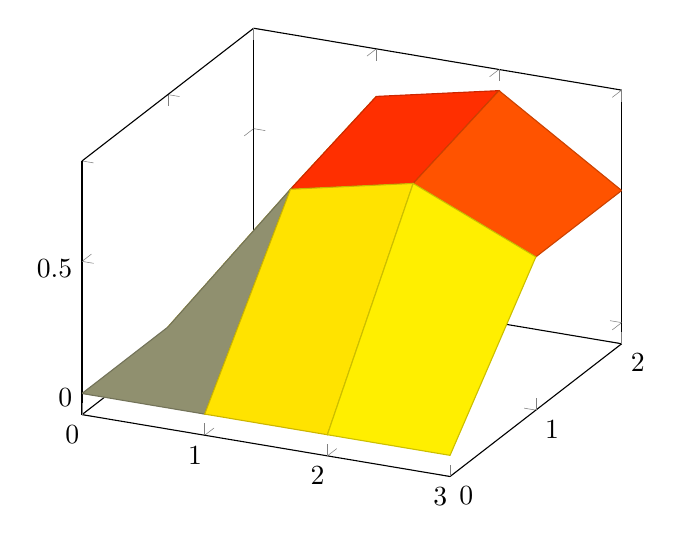
\begin{tikzpicture}
\begin{axis}
% this yields a 3x4 matrix:
\addplot3[surf]coordinates{
(0,0,0) (1,0,0) (2,0,0) (3,0,0)

(0,1,0) (1,1,0.6) (2,1,0.7) (3,1,0.5)

(0,2,0) (1,2,0.7) (2,2,0.8) (3,2,0.5)
};
\end{axis}
\end{tikzpicture}



\begin{tikzpicture}
\begin{axis}[xlabel=]
\addplot3[surf]table{plotdata/first3d.dat};
\end{axis}
\end{tikzpicture}